\chapter{Conclusions and Future Work}

\section{Conclusions}

Robotic MIS has a large impact in improving surgical operations while being demanding and complex in its implementation. Due to the nature of the tasks the surgical robots must execute, that is to operate on patients, the implemented solutions must have very strict requirements in accuracy and quality assurance. The critical requirements that were studied in this thesis are discussed in the sequel.\\

\textbf{Positional accuracy}: The trajectories that the robot executes (especially the pivot trajectories inside the surgical site) must be executed with micrometer accuracy. This positional accuracy is required for both the end-effector as well as for the tip of the surgical tool. It is important to note, that due to the fulcrum effect a small error in the end-effector can cause a larger error in the position of the tool tip and vice-versa. Errors larger than several micrometers can cause serious surgical side-effects. The experiments of this thesis were conducted with the requirement of bounding the position error of the end-effector to $\pm 5μm$. The positional accuracy in trajectories outside of the patient body is not as strict and was increased to $0.5mm$.\\

\textbf{Orientation accuracy}: Orientation accuracy is also very crucial for both the end-effector and the tip of the surgical tool, and it affects the deviation error from the fulcrum point. Orientation errors can also have negative side-effects in the surgical operation and small errors in the end-effector can cause bigger errors in the tool tip and vice-versa. The experiments of this thesis were conducted with the requirement of bounding the orientation error of the end-effector to $\pm 5\cdot 10^{-6}$degrees. The orientation accuracy in trajectories outside of the patient body, was increased to $\pm 5\cdot 10^{-4}$degrees.\\

\textbf{Time optimization}: Time optimal trajectories are concerned with finding the paths, avoiding collisions and respecting the constraints as well as calculating the trajectories in the shortest amount of time as possible. This is very important, so that the robot can be responsive in real-time to the surgeon’s commands and to be able to quickly and safely execute a given task. In all experiments a maximum of 5 seconds was specified for each path planning request. Although this time duration is significantly large, many experiment path planning requests were completed in less than a second (see measurements from \ref{section:robot-planner1}, \ref{section:robot-planner2}, \ref{section:robot-planner3b}).\\

\textbf{RCM constraint}: To satisfy the RCM constraint, all trajectories were designed using spherical coordinates with respect to the fulcrum reference frame. To make sure that the surgical tool satisfies this constraint an RCM error metric was used to measure the distance of the line of the long axis of the tool from the fulcrum point. This error was mostly measured for the insertion, retraction and line segment trajectories with very satisfactory results with the errors being in the magnitude of micrometers 
(see Figure~\ref{robot-planner3b-line-seg-rcm-errors}). It is important to keep this error at a minimum to avoid exerting pressure to the patient’s abdominal wall.\\

\textbf{Interpolation accuracy}: This requirement states that the number of interpolated waypoints of a path/trajectory should be enough such that the geometry of the path is not significantly distorted. In this thesis the interpolation is implemented in two stages; the first stage is the one related to creating distortionless trajectories and the second is a lower level interpolation made by MoveIt path planner when executing Cartesian line paths. For this second interpolation, a step distance is defined such that the actual executed path is as close to the line as possible (see Figure~\ref{interpolation-accuracy}). In the simulations, the geometric interpolation was made using 20 or 50 sample points and the second interpolation was made using a step size of 1mm. For both parameters, a higher choice is recommended for more precise movements but with an extra cost of heavier computational requirements.\\

\textbf{Collision avoidance}: Path planning algorithms must take into consideration the environment obstacles and execute trajectories around them without colliding with them. In most cases this requirement was automatically satisfied from the MoveIt framework, where it was specified that each kinematics solution should be collision-aware. The second case that was not handled by MoveIt and was separately handled in the experiments was the elbow-up constraint. This constraint (see also \ref{section-elbow-up-constraints}) was purposefully imposed so that the robot arm’s elbow would not collide with the mounting dock (the object with the trocars that simulates the patient) when executing pivot motions.\\

\textbf{Suitable path planning algorithms}: The MoveIt motion planning framework for ROS provides a wide range of path planning algorithms to choose from. The requirements for choosing a path planning algorithm were to find a collision-aware solution in the shortest time possible, respecting all constraints, without any replanning (if possible) and to provide under the same conditions the same results. In the first simulation study the two algorithms that were benchmarked were the RRTConnect and the RRT* algorithms and all other experiments were conducted using the RRTConnect algorithm, which provided satisfactory time results.\\

\textbf{Repeatability} \& deterministic results: When studying robotic applications another is the robot’s repeatability. The repeatability measures how “close” the measurements are with each other. A good repeatability is achieved when the measurements' standard deviation is as small as possible. In this thesis, all measurements were generated from running each simulation at least 10 times, in order to calculate the average and the standard deviation. Deterministic results in the measurements, in the context of this thesis, means that the measurements are not random and are predicted to be close to the average measurement and within a range of two or three standard deviations.\\

\textbf{Environment layout and robot base position}: Selecting the robot's position in the operating room and setting up the objects’ layout is quite important. The surgical tools’ positions that the robot must approach, and the surgical site, where the robot must operate at, must be fully inside the robot's workspace and be well reachable with ease and flexibility. In the first 2 simulations, a layout was used that made it difficult for the robot to reach all surgical tools and trocar points. In the remaining simulations a different layout was used, where the robot was much closer to the tools and the surgical site and could execute the pivot trajectories with more flexibility.\\

\textbf{Trajectory reachability}: The designed trajectories, especially those of the pivot motions, must be  in such a way so that the robot can fully follow them with ease and flexibility. The “flexibility” term means, to operate at points away from singularity points, away from the workspace boundary and without poses that make the robot to “self-fold” or even worse to self-collide.\\

\textbf{Singularity avoidance}: When in a singularity point, the robot loses one or more kinematic DoF and moving it would require large effort from the joints. This can result in surgical side-effects, as well as cause problems to the robot and should always be avoided. Singularity points are avoided from the MoveIt framework when calculating the paths, and are also avoided in the lower-level controllers of the robot’s  hardware. Singularity point approaching was also tracked using the robot’s Jacobian and the manipulability index (see Figure~\ref{robot-planner1-manipulability-plot}).\\

\textbf{Jump threshold}: This parameter reduces the large unpredictable motions of redundant joints that could be a safety issue (in this case both for the patient and the operating staff). These undesirable motions can occur when the arm approaches singularities and needs to reorient the arm in order to continue following the trajectory. In simulation experiments this parameter was disabled to better study the path planning in all possible cases.\\

The aforementioned conclusions were drawn given the following \textbf{assumptions} that were taken into consideration to simplify, without loss of generality, certain simulation studies. 
\begin{itemize}
\item The \textbf{fulcrum position and orientation} were assumed known and constant. All trajectories from the simulations were calculated using constant fulcrum reference frames, which according to the bibliography in more realistic scenarios is not the case, and the pose of a fulcrum point is usually estimated.
\item The surgical tool appears fixed on the end-effector of the robot. In this thesis a higher level overview of \textbf{surgical tool grasping} was studied in order to better study the pivot trajectories separately without being affected by grasping forces and fulcrum-tool torques.
\item The simulation environment features were assumed known and constant, which means that the pose of the surgical tools and the trocar were assumed known and their values were not extracted from the \textbf{Computer Vision node} that calculated these poses using a stereoscopic camera.
\end{itemize}

The goal of this thesis was to study in an \textbf{end-to-end approach}, all the stages involved in the perception, control and manipulation of laparoscopic tools, but \textbf{more emphasis was given to the pivot 
trajectories and the RCM constrained motion planning}. Since this approach is very complex and involves many different algorithms, mathematics, techniques and technologies, it was very useful that each stage was studied separately and self-isolated to ensure that each stage performs well on its own (unit testing), so that later all stages can be integrated and studied together (integration testing). A higher level end-to-end pipeline that can be used for integration testing is proposed in the state machine of \ref{section:robot-planner7}. \\
%
\section{Future Work}
%
\textbf{Simulation and interaction with deformable bodies}. 
In this thesis the laparoscopic tool is inserted through holes (trocars) in a mounting dock that simulates the patient. A more realistic approach would be instead of using such a rigid mounting dock, to use a deformable phantom object to study the interaction between the laparoscopic tool, the trocar and the patient's abdominal wall. Such a simulation is not feasible using ROS Gazebo simulation environment because it does not support collisions and physics with deformable objects. A framework that could be used with the help of a suitable ROS plugin to simulate deformable objects is the SOFA Framework.
%
\begin{center}
\begin{figure}[!htb]
\centering
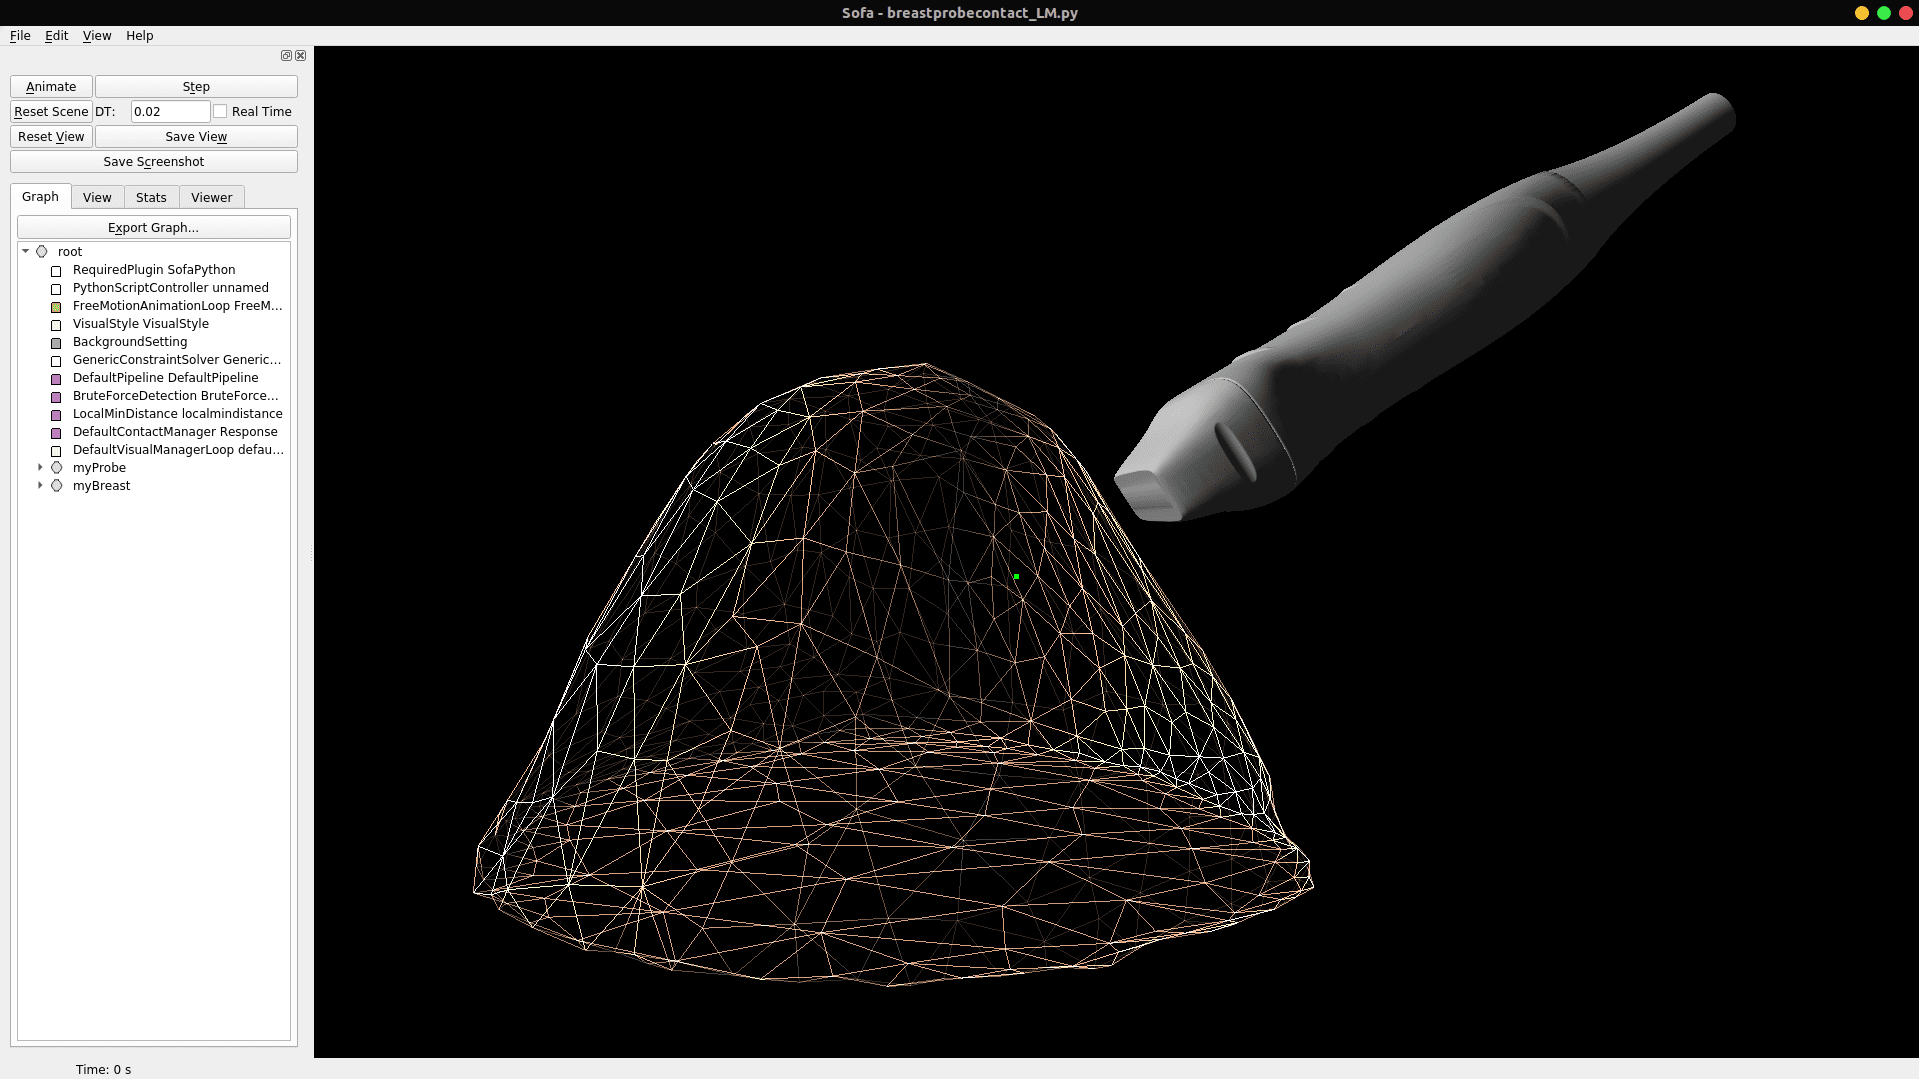
\includegraphics[width=0.35\textwidth]{images/future-work-sofa1.png}
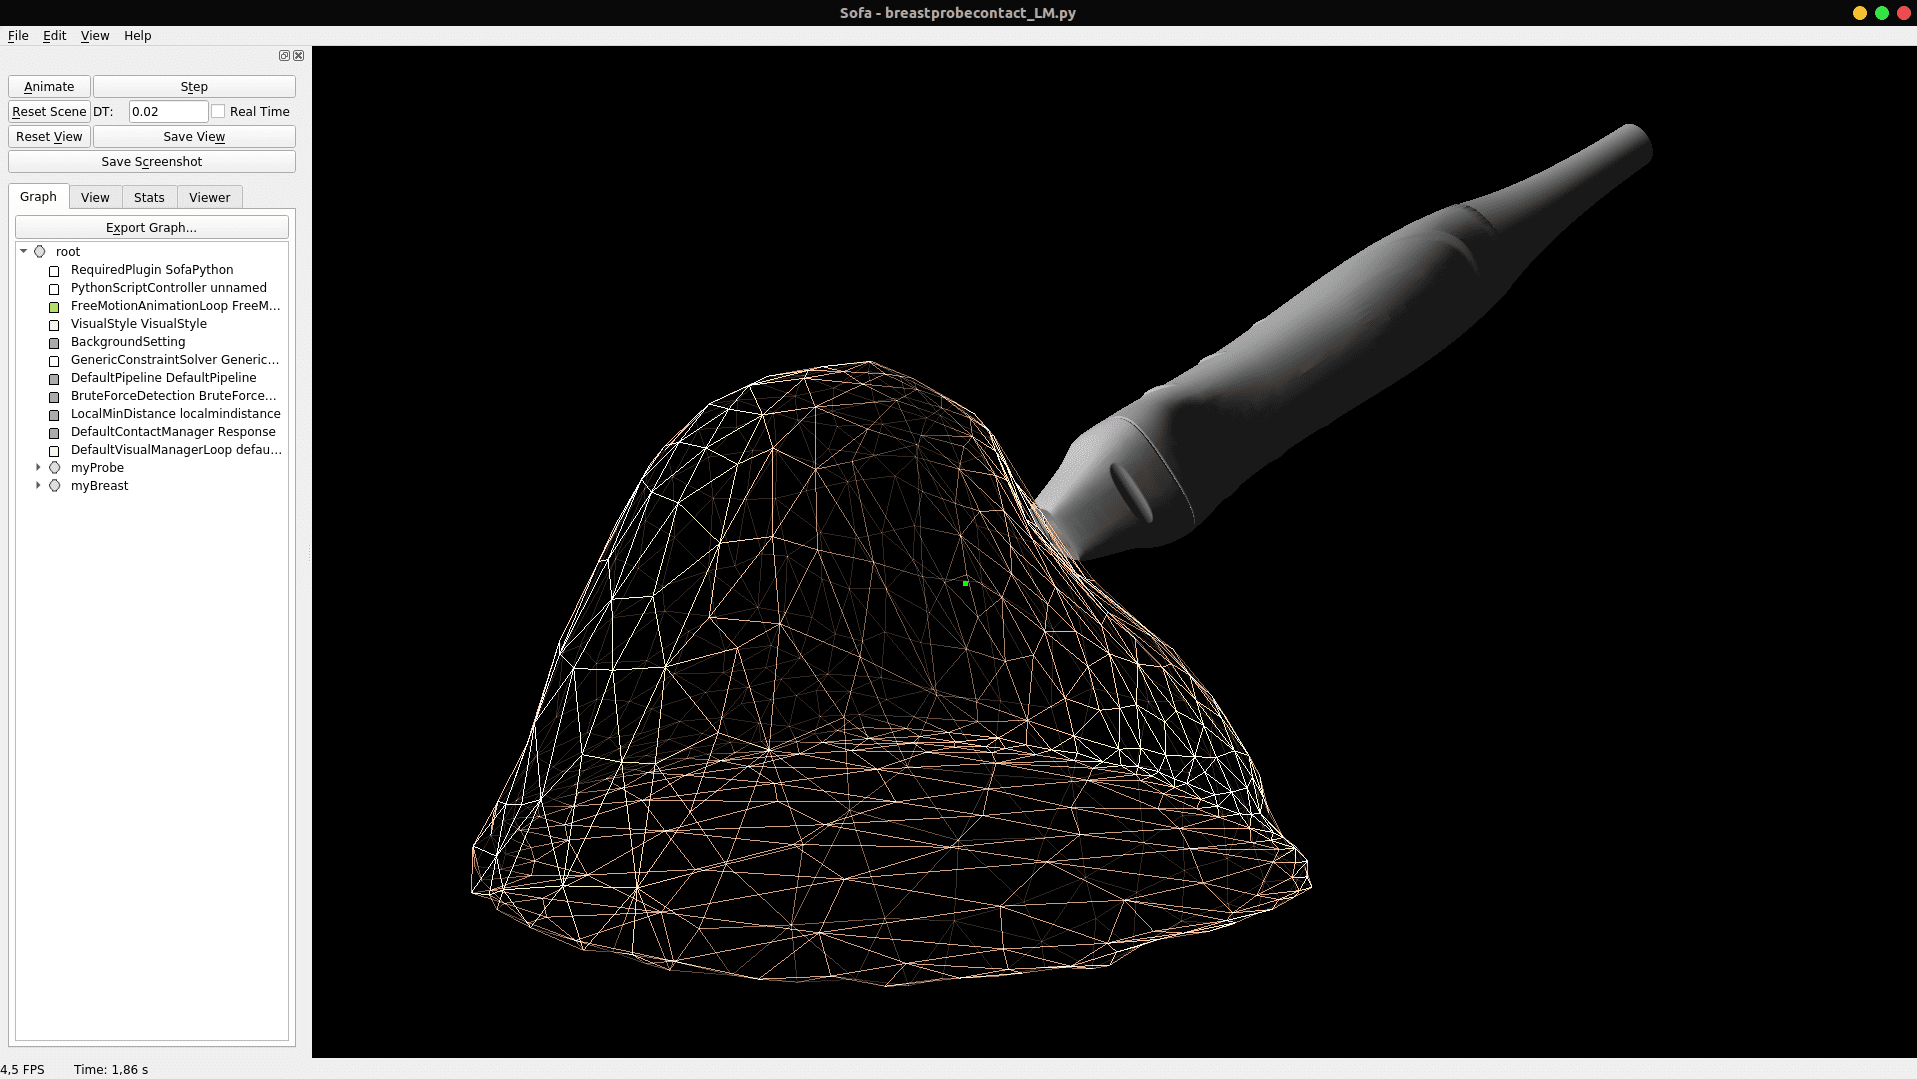
\includegraphics[width=0.35\textwidth]{images/future-work-sofa2.png}\\
\caption{Deformable tissue/organ medical simulation - Simulation of breast probing using the SOFA Framework. Screenshots from running the repository at
\url{https://gitlab.com/altairLab/probe-tissue-simulation}}
\end{figure}
\end{center}

\textbf{Advanced visualization and Haptics feedback}
In this thesis, no medical imaging is used relevant to laparoscopic operations. It would be greatly beneficial to study pivot motions based on medical imaging or haptic feedback from endoscopic instruments. CHAI3D is an open source, platform agnostic framework for computer haptics, visualization and interactive real-time simulation which supports haptic devices.
%
\begin{center}
\begin{figure}[!htb]
\centering
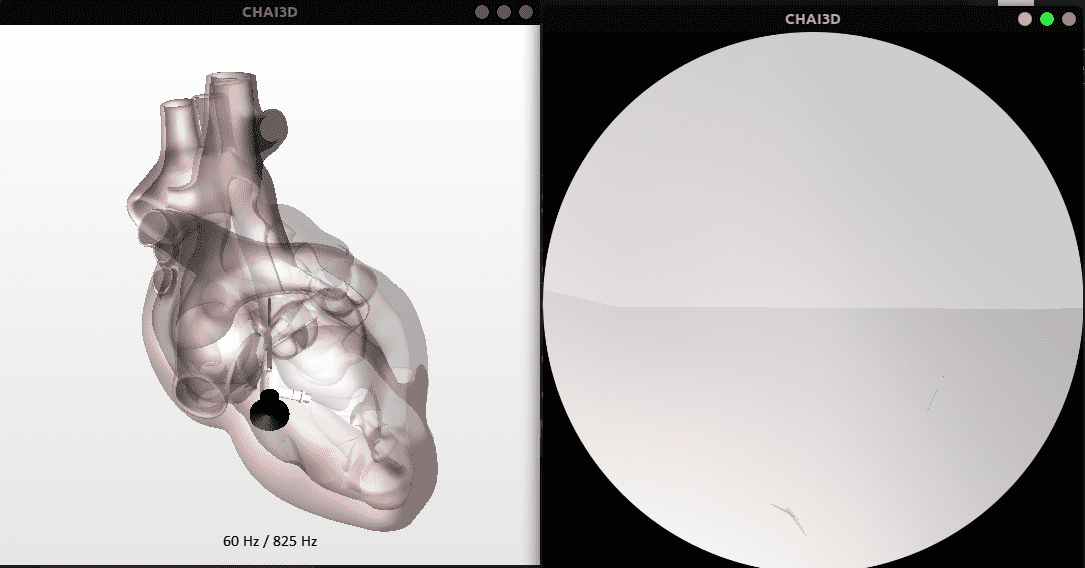
\includegraphics[width=0.7\textwidth]{images/future-work-chai3d.png}\\
\caption{Heart endoscopy medical simulation using the CHAI3D framework. Screenshots from running the repository at
\url{https://github.com/chai3d/chai3d}}
\end{figure}
\end{center}


Other ideas for future work that could improve and further explore the outcomes of this thesis are:
\begin{itemize}
\item Using the trajectories from Chapter~\ref{chapter-6} as building blocks for more complicated trajectories like suturing or cauterization
\item Design pivot trajectories without assuming that the Fulcrum point is known and constant and use estimation methods (like a Kalman filter) to estimate its pose
\item Multiple robot arm collaboration: designing pivot trajectories for two or more robot arms that collaborate for a common surgical task, for example one robot controls an endoscopic camera and the other robot controls the surgical tools
\item Applications of Machine Learning in Computer Vision: detection of laparoscopic tools
\end{itemize}
